\subsection {ROC}

\acrfull{roc} is a reconfigurable optical wavelength \\ \gls{co-processor}, implemented in two distinct physical technologies, capable of approximately solving \acrshort{pde}s through the \gls{finite difference method}, constructed in a physical analog mesh but differing from the electrical implementation introduced in Figure \ref{fig:01_analytical_numerical_analog} by performing summation of electrical \gls{displacement current} desnity for \gls{Metatronic} \acrshort{roc} and summation of \gls{optical intensity} in \gls{Photonic} \acrshort{roc}. 

\par Increases in the \gls{RC time constant} as a 2D electric mesh scales its number of nodes quadratically increases signal delay across the diameter of the mesh. If this signal delay exceeds the clock speed of the processor the computational time complexity of the analog electrical mesh degrades from $O(1)$ to $O(n)$ where $n$ is the number of nodes along a single side of a square mesh.

\par Different electrical meshes, as shown in Figure \ref{fig:01_analytical_numerical_analog}, must be fabricated for different configurations of \acrshort{pde}s, therefore making an electronic analog static co-processor non reconfigurable.

\par Static photonic \acrshort{roc} utilizes changes in optical intensity due to optical loss to solve Laplace and Poisson \acrshort{pde}s. \gls{Metatronic} \acrshort{roc} confines electric displacement current density $J_D = \frac{\partial D}{\partial t}$ in epsilon vary large (EVL) materials surrounded by epsilon near zero (ENZ) materials and directs $J_D$ through nano-inductors, nano-capacitors, and nano-resistors.

\par The ability to change the accuracy of the \acrshort{pde} solution through the ratio of the density of the mesh versus the area of the \acrshort{pde} being solved for makes the \acrshort{roc} co-processor concept appropriate for future Energy-Quality (EQ) scalable systems, advocated for by  green computing initiatives, which require the ability to explicitly trade off energy and quality at different levels of abstraction \cite{M.Alioto_2017}.

\begin{figure}[ht]
\centering\fbox{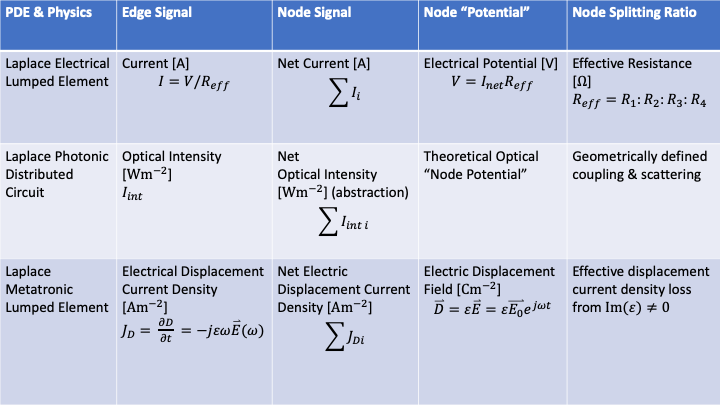
\includegraphics[height=3.5in, width=6in]{figures/figures1/02b_physics_table.png}}
\caption{The Laplace \acrshort{pde} dependent physical units and equations for grid components in the electronic mesh, photonic \acrshort{roc}, and metatronic \acrshort{roc} are shown. The electrical and metatronic circuits operate as lumped elements and the photonic circuit operates as a distributed circuit. The equation units of metatronic \acrshort{roc} electric displacement current density are as follows: $\tilde{\varepsilon}$ material permittivity [\si{\farad \meter^{-1}}], $\omega = 2\pi f$ Angular Frequency [\si{\hertz}], $E(\omega)$ electrical field [\si{\volt \meter^{-1}}] or [\SI{}{\newton \coulomb^{-1}}]. It is also important to distinguish between which photonic quantity's are measurable. We measure optical intensity through the use of a Y branch and a grating along each edge at the output of each optical node.}
\label{fig:01_02b_physics_table}
\end{figure}


\subsection{Photonic}

\par Passive photonic ROC utilizes pure etched silicon waveguides and ring resonators combined with an central splitting element combined to form a photonic device that directs light evenly from the input port to the 3 output ports with a 33.3\% 33.3\% 33.4\%  splitting. Photoinc ROC is fabricated within the GW clean room and is at a length scale greater than the wavelength of light, $\lambda = \SI{1550}{n\meter}$ being using. The distance form node to node is $h = \SI{60}{u\meter}$. This size differential results in Photoinc ROC operating in accordance to the \gls{distributed element model} shown in Figure \ref{fig:01_02_electrical_photoinc_metatronic}. 

\par Unfortunately there is a weak mapping of the electrical mesh to the photonic Mesh. This is because we must attempt to replicate electrical resistance with optical loss which is not equivalent. We also do not have a photonic equivalent to electrical capacitance or electrical inductance. However due to the relative ease of manufacturing a photonic mesh compared to a metatronic mesh we have invested energy and time into the photonic implementation of ROC as a way to demonstrate an initial fabrication. However the combination of equal splitting along with the distributed element model means that as we scale ROC for larger numbers of nodes the overall accuracy of the PDE solution decreases which is the opposite of what is desired for a analog finite difference algorithm as it is scaled up as noted in Figure \ref{fig:1_03a_elec_accuracy}.

\begin{figure}[ht]
\centering\fbox{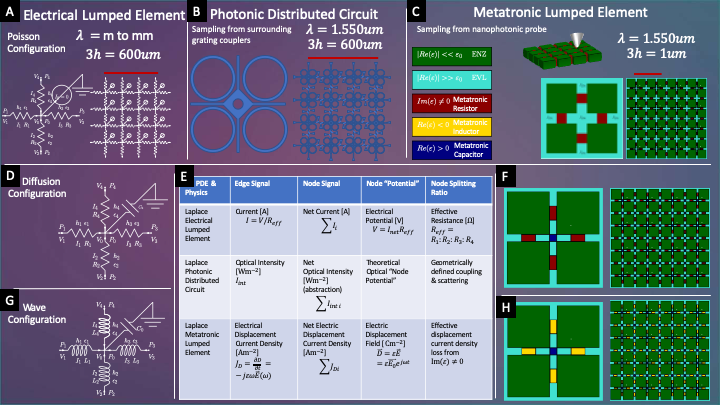
\includegraphics[height=3.5in, width=6in]{figures/figures1/02_electrical_photonic_metatronic.png}}
\caption{ The top row of this figure illustrates the different analog grid based \acrshort{pde} solving technologies including \textbf{(A)} the original electrical analog, \textbf{(B)} the silicon photonics implementation, and \textbf{(C)} the Metatronic Implementation. The columns represent the different configurations of the grid, that give the “reconfigurable” optical computer its name, allowing for Poisson, diffusion, and wave configurations. 
As you probably have noticed, there is no photonic schematic showing an equivalence to \textbf{(D)} electrical capacitance, or \textbf{(G)} electrical inductance, but there is \textbf{(F)} metatronic capacitance and \textbf{(H)} metatronic inductance. Table \textbf{(E)} shows the physical effects utilized in the technologies and is shown in larger form in Figure \ref{fig:01_02b_physics_table}. In the language of graph theory, a node is a grid point within the mesh, and an edge is a connection between grid points.}
\label{fig:01_02_electrical_photoinc_metatronic}
\end{figure}

\subsection{Metatronic}

\par In microelectronics and combination of an electrical current and electrical potential through lumped elements including resistors, inductors, and capacitors has led to successful modularization of circuit design through the radio frequency and microwave domains. As we have seen in the photonic case, operating in the optical domain while still benefiting from a lumped circuit paradigm is not trivial. As Nadar Engatar stated in his 2007 Science paper \cite{N.Engheta_2007} there are two primary challenges to overcome. In lower frequency domains, designs involve elements that are much smaller than the wavelength of operation, fabrication techniques can be used to construct sub wavelength dimensions at optical wavelengths. Secondly the response of metals at IR and optical frequencies cannot be scaled directly from RF to optics.

\par The ideal metamaterial-based implementation of ROC with epsilon near zero set equal to zero as well as physically possible epsilon near zero values are simulated in the \gls{COMPSOL Multiphysics} based metatronic solution. of \acrshort{roc}.  Upper bounds are placed on the accuracy by $\lambda/L$, where $L$ is the feature size of the network components, due to the physical nature of light, and $\lambda$ is the wavelength.  

\par Metatronics enable the ideal ROC implementation, in terms of size and accuracy. However, the complexities of an effective integration of a high speed programmable and concurrently energy efficient static-like analog mesh significantly reduced the advancement of this technology.  Here, we demonstrate the implementation of a nano-optic co-processor able to solve partial differential equation based on a metatronic nanocircuit board. 

\par Thanks to a unprecedented control of the \acrfull{enz} and material losses over \gls{Indium tin oxide} (\acrshort{ito}), we use different deposition conditions, in order to tune the \acrshort{enz} position, which potentially leads to a top-down monolithically integrated circuit \cite{gui2018impact}. The elements of the circuit could be then be electrostatically tuned \cite{amin20180, ma2015indium, alu2018metasurfaces, tahersima2017testbeds} and reprogrammable aiming to solve a variety of PDEs including Poisson, diffusion, and wave. 

\par A discussion on losses and physical limitation, induced by the losses of the ITO at ENZ condition is provided. The solution accuracy and its scaling functions are estimated for to finite difference approaches, and compared to other mesh solutions. The implementation of an all optical read-out paradigm is discussed based on a Nanophotonic \gls{probe card} that detects the local near field of the scattered field and provides information of a dielectric displacement, at given points of the nano-optics circuit, thus allowing to extrapolate the results of the computation. 
